%\documentclass[hidelinks, conference]{IEEEtran}
\documentclass[hidelinks, 11pt, twocolumn]{article}
\usepackage{graphicx}
\usepackage{amssymb}
\usepackage{epstopdf}
\usepackage{blindtext}
\usepackage{hyperref}
\usepackage[document]{ragged2e}


\setlength{\columnsep}{1cm}
\setlength{\parskip}{.65em}
%=====================================================================================================

\begin{document}

\title{\textbf{Learning How to Use BibTeX}}
\author{Dr. Author}
\date{2021}
\maketitle


\tableofcontents

\begin{abstract}

	Using a dedicated .bib file is the best way to do references.
	You can map the citations to a string (foo-bar-86 in this case) that contains values related to the written work.
	If you use bibitems, especially without labels - meaning you must reference by index - references can be hard to keep track of.
	Here is a citation from a template for illustrative purposes.
	\cite{foo-bar-86}

\end{abstract}
\pagebreak


\section{Introduction}


Here is an example of a BibTeX entry for a book.

\begin{flushleft}
	\textit{@Book\{taleb2005fooled,}\\
	\hspace{1em} \textit{author = \{Taleb, Nassim\},}\\
	\hspace{1em} \textit{title = \{Fooled by randomness : the hidden role of chance in life and in the markets\},}\\
	\hspace{1em} \textit{publisher = \{Random House\},}\\
	\hspace{1em} \textit{year = \{2005\},}\\
	\hspace{1em} \textit{address = \{New York\},}\\
	\hspace{1em} \textit{isbn = \{0-8129-7521-9\}}\\
	\textit{\}}
\end{flushleft}

You can create BibTeX references from an ISBN with this site.

\url{https://www.ottobib.com/}

If an article has a DOI (digital object identifier, used to identify journal articles) then you can use this API to get BibTeX references.

\url{http://api.crossref.org/works/REPLACE-ME-WITH-DOI/transform/application/x-bibtex}


For example, here is Einstein's 1905 paper on Brownian Motion using that method.

\url{http://api.crossref.org/works/doi:10.1002/andp.19053220806/transform/application/x-bibtex}



\section{Everything is Luck}

\begin{figure}[h]
	\centering
	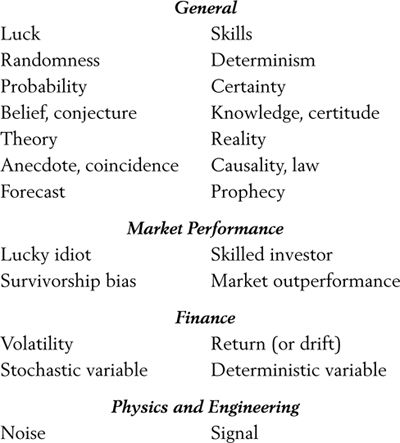
\includegraphics[scale=1]{images/luck-skill.jpg}\\
	\caption{People tend to attribute the left to the right. \cite{taleb2005fooled}}
	\label{fig:how_pop3_works}
\end{figure}

\textit{This book is about luck disguised and perceived as nonluck (that is, skills) and, more generally, randomness disguised and perceived as non-randomness (that is, determinism).
	It manifests itself in the shape of the lucky fool, defined as a person who benefited from a disproportionate share of luck but attributes his success to some other, generally very precise, reason.
	Such confusion crops up in the most unexpected areas, even science, though not in such an accentuated and obvious manner as it does in the world of business.
	It is endemic in politics, as it can be encountered in the shape of a country’s president discoursing on the jobs that “he” created, “his” recovery, and “his predecessor’s” inflation.\cite{taleb2005fooled}}


That is the lens Nassim Taleb uses to analyze the world, concisely stated as the first paragraph of the prologue of his first book
- \textit{Fooled by Randomness: The Hidden Role of Chance in Life and in the Markets}.



\section{Brownian Motion Citation Example}
\blindtext \cite{Einstein_1905}

\section{Sokal Affair Example}
\blindtext[5] \cite{Sokal_1996}

\pagebreak
\bibliographystyle{IEEEtran}
\bibliography{paper}

\end{document}
